\documentclass[tikz]{beamer}

\usepackage{tikz}
\usetikzlibrary{shapes,arrows}
\mode<presentation>{}
\usepackage{beamerthemeshadow}

%\usepackage{pseudocode}
%\usepackage{dirtree}
% \usepackage[utf8]{inputenc}
% \usepackage{listings,xcolor}

% \usepackage{soul}
% \usepackage{ulem}


\usepackage{tikz-cd}
\usepackage{amsmath}
\usepackage[most]{tcolorbox}


\DeclareMathOperator*{\argmin}{arg\,min}


\usepackage[linesnumbered,lined,boxed,commentsnumbered]{algorithm2e}
%\usepackage{algorithmicx}
\usepackage{algpseudocode}
\algrenewcommand\algorithmicwhile{\textbf{until}}
\SetKwInOut{Input}{input}
\SetKwInOut{Output}{output}



\usepackage[round,authoryear]{natbib}
%\usepackage[margin=1.0in]{geometry}
\usepackage{graphicx}
\usepackage{moreverb}
\usepackage{hyperref}
\newcommand\infNorm[1]{\left\lVert#1\right\rVert_\infty}
\newcommand\twoNorm[1]{\left\lVert#1\right\rVert_2}
\newcommand\someNorm[1]{\left\lVert#1\right\rVert}

\usepackage{mathtools}
\mathtoolsset{showonlyrefs}

\usepackage[english]{babel}
\usepackage[12hr,level]{datetime}
%\usepackage{datetime}
\usepackage{amsfonts}

\newcommand{\xgusst}[1]{x^{guess}_{#1}}
\newcommand{\xnxt}[1]{x^{next}_{#1}}
\newcommand{\znxt}[1]{z^{next}_{#1}}
\newcommand{\xlst}[1]{x^{last}_{#1}}
\newcommand{\zlst}[1]{z^{last}_{#1}}
\newcommand{\zgusst}[1]{z^{guess}_{#1}}
\newcommand{\xguss}{\xgusst{}}
\newcommand{\xtpguss}{x^{tp1guess}}


\newcommand{\iSet}{{\mathcal{I}_t}}

\newcommand{\posInt}{{\mathcal{N}^+}}
\newcommand{\Rn}[1]{{\mathcal{R}^{#1}}}
\newcommand{\numX}{{N_x}}
\newcommand{\numZ}{{N_z}}
\newcommand{\numEps}{{N_\epsilon}}
\newcommand{\numR}{{N_r}}
\newcommand{\numIters}{{K}}
\newcommand{\numTerms}{{N_{terms}}}
\newcommand{\numPts}{{N_{points}}}
\newcommand{\thePoints}{{\{(x_{t-1},\epsilon_t)^{1} \ldots (x_{t-1},\epsilon_t)^{\numPts}\}}}
\newcommand{\thePts}{{\mathcal{P}}}
%\newcommand{\ADRCE}{{\bf ADRCE}}
%\newcommand{\ADR}{{\bf ADR}}
\newcommand{\ADRCE}{\XZFunc}
\newcommand{\ADR}{\xzFunc}




\newcommand{\xtmEpsArg}{{x_{t-1},\epsilon_t}} 
\newcommand{\xtArg}{{x_{t} }}


\newcommand{\sumLinPart}{{
B x_{t-1}+ \phi \psi_\epsilon\epsilon + (I - F)^{-1} \phi \psi_c 
}}
\newcommand{\sumZPart}{{
 \sum_{\sForSum=0}^\infty F^s \phi z_{t+\sForSum}(x_{t-1},\epsilon) 
}}
\newcommand{\sumZPartZero}{{
 \phi z_{t}(x_{t-1},\epsilon) 
}}
\newcommand{\sumZPartPos}{{
 \sum_{\sForSum=1}^\infty F^s \phi Z_{t+\sForSum}(x_{t-1},\epsilon) 
}}

\newcommand{\EsumLinPart}{{
	 B x_{t-1}+ (I - F)^{-1} \phi \psi_c 
}}
\newcommand{\EsumZPartZero}{{
	  \sum_{\sForSum=0}^\infty F^s \phi Z^{PF}_{t+\sForSum}(x_{t-1},0) 
}}
\newcommand{\EsumZPartEpsilon}{{
	  \sum_{\sForSum=0}^\infty F^s \phi \expct{z_{t+\sForSum}(x_{t-1},\epsilon)}
}}
\newcommand{\EsumCapZPart}[1]{{
	  \sum_{\sForSum=0}^\infty F^s \phi {Z^{#1}_{t+\sForSum}(x_{t-1})}
}}
\newcommand{\uncnxpt}[2]{{\mathcal{E}\left [ \left . #1 \right | #2  \right ]}}
\newcommand{\expct}[1]{{\mathcal{E}\left [ #1 \right ]}}

\newcommand{\xzFuncGuess}{{\mathbb{g}}}
\newcommand{\xzFuncGuessIn}{{\mathbf{\mathbb{g}_{in}}}}
\newcommand{\genxzFuncGuessIn}{{\mathbf{gen\mathbb{g}_{in}}}}
\newcommand{\xzFuncGuessSig}{{(\Rn{\numX})\rightarrow
(\Rn{({\numX+\numZ})})}}


\newcommand{\xzFunc}{{{\gamma}}}
\newcommand{\xzFuncSig}{{(\Rn{\numX+\numEps})\rightarrow
(\Rn{({\numX+\numZ})})}}

\newcommand{\XZFunc}{{\mathbb{G}}}
\newcommand{\genXZFunc}{{\mathbf{gen\mathbb{G}}}}
\newcommand{\bigXFuncSig}{{(\Rn{\numX})\rightarrow
(\Rn{({\numX+\numZ})})}}


\newcommand{\genXGFP}{{\mathcal{U}}}
\newcommand{\xgFP}{{\mathcal{V}}}

\newcommand{\genFpf}{{\mathbf{gen}_\fpf}}
\newcommand{\fpf}{{\mathcal{T}}}
\newcommand{\fpfIn}{{\mathbf{t}_{in}}}
\newcommand{\fpfOut}{{\mathbf{t}_{out}}}
\newcommand{\genFpfIn}{{\mathbf{gen\fpf}_{in}}}
\newcommand{\genFpfOut}{{\mathbf{gen\fpf}_{out}}}

\newcommand{\genSlvr}{{\mathbf{gen}_{\slvr}}}
\newcommand{\slvr}{{\mathcal{S}}}
\newcommand{\slvrIn}{{\mathbf{s}_{in}}}
\newcommand{\slvrOut}{{\mathbf{s}_{out}}}
\newcommand{\genSlvrIn}{{\mathbf{gen\slvr}_{in}}}
\newcommand{\genSlvrOut}{{\mathbf{gen\slvr}_{out}}}
\newcommand{\solverSig}{{
\frfpnsRegimeFuncHelp
}}
\newcommand{\allArgs}{(x_{t-1},\epsilon,x_t,\expct{x_{t+1}})}
\newcommand{\proj}[1]{{\pi_{#1}}}
\newcommand{\eqnArg}{\mathbf{m}_{in}}
\newcommand{\eqnOut}{\mathbf{m}_{err}}
\newcommand{\eqnFunc}{\mathbb{M}}
\newcommand{\gate}{\mathbf{b}}
\newcommand{\eqnFuncSysIExpl}[1]{\{(\mathbf{b}_{#1}\allArgs,\eqnFunc_{#1}\allArgs=0) \}}
\newcommand{\eqnFuncSysI}[1]{\mathbb{C}_{#1}}
\newcommand{\eqnFuncSys}{\{\eqnFuncSysI{1},\ldots,\eqnFuncSysI{M}\}}
\newcommand{\eqnErrs}{{{m}_e}}
\newcommand{\eqnFuncSig}{{\Rn{3\numX+\numEps+\numZ}\rightarrow\Rn{\numX}}}


\newcommand{\lilXFuncSig}{{fix lilXFuncSig}}



\newcommand{\frfpnsFuncSig}{{\Rn{\numX+\numEps}\rightarrow\Rn{\numX+\numZ}}}

\newcommand{\bigXRegimeFuncSig}{{(\Rn{\numX+1})\rightarrow
(\Rn{({\numX+\numZ})})}}
\newcommand{\lilXRegimeFuncSig}{{(\Rn{\numX+1+\numEps+\numZ})\rightarrow
(\Rn{({3(\numX+1)+\numEps+\numZ})})}}
\newcommand{\eqnRegimeFuncSig}{{
\{\Rn{3(\numX+1)+\numEps+\numZ}\rightarrow\Rn{\numX},
\ldots,
\Rn{3(\numX+1)+\numEps+\numZ}\rightarrow\Rn{\numX}\}
}}
\newcommand{\frfpnsRegimeFuncHelp}{{\Rn{\numX+\numEps}\rightarrow\Rn{\numX+\numZ}}}

\newcommand{\frfpnsRegimeFuncSig}{{
\{ (\frfpnsRegimeFuncHelp{1}), \ldots ,  (\frfpnsRegimeFuncHelp{\numR})\}
}}

\newcommand{\dstSpec}{{\mathbf{distSpec}}}
\newcommand{\expctSpec}{{\mathbf{expctSpec}}}
\newcommand{\grdSpec}{{\mathbf{grdSpec}}}


\newcommand{\linMod}{{\mathcal{L}}}
\newcommand{\linModMats}{{\{H,\psi_\epsilon,\psi_c;B,\phi,F\}}}
\newcommand{\sForSum}{{\nu}}

\newcommand{\xWOarg}{   \mathbf{x}}
\newcommand{\xWarg}{   \mathbf{x}(x_{t-1},\epsilon)}
\newcommand{\xWargK}{   \hat{\mathbf{x}}(x_{t-1},\epsilon,k)}
\newcommand{\xWOargK}{   \hat{\mathbf{x}}}

\newcommand{\xpWOarg}{   \mathbf{x}^p}
\newcommand{\xpWarg}{   \mathbf{x}^p(x_{t-1},\epsilon)}
\newcommand{\xpWargK}{   \hat{\mathbf{x}}^p(x_{t-1},\epsilon,k)}
\newcommand{\xpWOargK}{   \hat{\mathbf{x}^p}}


\newcommand{\xppWOarg}{   \mathbf{x}^{p'}}
\newcommand{\xppWarg}{   \mathbf{x}^{p'}(x_{t-1},\epsilon)}
\newcommand{\xppWargK}{   \hat{\mathbf{x}}^{p'}(x_{t-1},\epsilon,k)}
\newcommand{\xppWOargK}{   \hat{\mathbf{x}^{p'}}}



\newcommand{\XWOarg}{   \mathbf{X}}
\newcommand{\XWarg}{   \mathbf{X}(x_{t-1},\epsilon)}
\newcommand{\XWargK}{   \hat{\mathbf{X}}(x_{t-1},\epsilon,k)}
\newcommand{\XWOargK}{   \hat{\mathbf{X}}}


\newcommand{\XpWOarg}{   \mathbf{X}^p}
\newcommand{\XpWarg}{   \mathbf{X}^p(x_{t-1},\epsilon)}
\newcommand{\XpWargK}{   \hat{\mathbf{X}^p}(x_{t-1},\epsilon,k)}
\newcommand{\XpWOargK}{   \hat{\mathbf{X}^p}}

\newcommand{\zWOarg}{   \mathbf{z}}
\newcommand{\zWarg}{   \mathbf{z}(x_{t-1},\epsilon)}
\newcommand{\zWargK}{   \hat{\mathbf{z}}(x_{t-1},\epsilon,k)}
\newcommand{\zWOargK}{   \hat{\mathbf{z}}}


\newcommand{\ZWOarg}{   \mathbf{Z}}
\newcommand{\ZWarg}{   \mathbf{Z}(x_{-1},\epsilon)}
\newcommand{\ZWargK}{   \hat{\mathbf{Z}}(x_{-1},\epsilon,k)}
\newcommand{\ZWOargK}{   \hat{\mathbf{Z}}}


\newcommand{\zpWOarg}{   \mathbf{z}^p}
\newcommand{\zpWarg}{   \mathbf{z}^p(x_{t-1},\epsilon)}
\newcommand{\zpWargK}{   \hat{\mathbf{z}^p}(x_{t-1},\epsilon,k)}
\newcommand{\zpWOargK}{   \hat{\mathbf{z}^p}}



\newcommand{\zppWOarg}{   \mathbf{z}^{p'}}
\newcommand{\zppWarg}{   \mathbf{z}^{p'}(x_{t-1},\epsilon)}
\newcommand{\zppWargK}{   \hat{\mathbf{z}^{p'}}(x_{t-1},\epsilon,k)}
\newcommand{\zppWOargK}{   \hat{\mathbf{z}^{p'}}}


\newcommand{\ZpWOarg}{   \mathbf{Z}^p}
\newcommand{\ZpWarg}{   \mathbf{Z}^p(x_{-1},\epsilon)}
\newcommand{\ZpWargK}{   \hat{\mathbf{Z}^p}(x_{-1},\epsilon,k)}
\newcommand{\ZpWOargK}{   \hat{\mathbf{Z}^p}}


\newcommand{\xIter}[2]{\mathcal{X}^{#1}(#2)}
\newcommand{\xNow}[1]{x^{#1}_t(x_{t-1},\epsilon_t)}
\newcommand{\zNow}[1]{z^{#1}(x_{t-1},\epsilon_t)}
\newcommand{\xNowtp}[1]{x^{#1}_{t+1}(x_{t-1},\epsilon_t)}
\newcommand{\XNow}[3]{\mathcal{X}^{#1}_{#2}(x_{#3})}
\newcommand{\ZNow}[3]{\mathcal{Z}^{#1}(x_{#3})}


\newcommand{\rcpC}{{\mathbf{N}}}


\newcommand{\gssaKtp}{{\left \{  
\beta \frac{u^\prime(c_{\tau+1})}{u^\prime(c_{\tau})} 
[1- \delta + a_{t+1}f^\prime(k_{\tau+1})]
\right \} -1}}


\newenvironment{myProof}[1][Proof]{\begin{trivlist}
  \item[\hskip \labelsep {\bfseries #1}]}{\end{trivlist}}
\newenvironment{myDefinition}[1][Definition]{\begin{trivlist}
\item[\hskip \labelsep {\bfseries #1}]}{\end{trivlist}}
\newenvironment{myExample}[1][Example]{\begin{trivlist}
\item[\hskip \labelsep {\bfseries #1}]}{\end{trivlist}}
\newenvironment{myRemark}[1][Remark]{\begin{trivlist}
\item[\hskip \labelsep {\bfseries #1}]}{\end{trivlist}}

\newcommand{\myQed}{\nobreak \ifvmode \relax \else
      \ifdim\lastskip<1.5em \hskip-\lastskip
      \hskip1.5em plus0em minus0.5em \fi \nobreak
      \vrule height0.75em width0.5em depth0.25em\fi}

\newcommand{\xtFuncTI}{\mathcal{X}(x,\epsilon)}
\newcommand{\XtFuncTI}{\mathbf{X}(x)}
\newcommand{\expctEps}[1]{\mathcal{E}_{\epsilon} \left [#1 \right ]}
\newcommand{\xsubtFunc}[2]{\mathcal{X}_{#1}{#2}}
\newcommand{\xtFunc}[1]{\mathcal{X}{#1}}
\newcommand{\XtFunc}[1]{\mathbf{X}{#1}}
\newcommand{\stochF}[1]{\mathcal{S}^{\{#1\}}}
\newcommand{\detF}[1]{\mathcal{D}^{\{#1\}}}
\newcommand{\initXE}{(x_{-1},\epsilon_0)}
\newcommand{\nlEqnLHS}[4]{
  h_\varpi(#1,#2,E_t(#3),\epsilon_#4)}

\newcommand{\nlEqn}[4]{
h_\varpi^{det}(#1,#2,\epsilon_#4)+
H_\varpi^{det}(#1,#2,\epsilon_#4)E_#4(#3)
}
\newcommand{\nlEqnSel}[4]{
\varpi=m_\varpi^{det}(#1,#2,\epsilon_#4)+
M_\varpi^{det}(#1,#2,\epsilon_#4)E_#4(#3)
}
\newcommand{\itSup}[1]{{\{#1\}}}
\newcommand{\initX}{(x)}
\newcommand{\initXEN}{(x_,\epsilon_t)}
\newcommand{\detComp}[1]{{\detF{K-\nu}( \cdots \detF{K-1}(\detF{K}(#1))))}}
\newcommand{\tArg}{(x_{t-1},\epsilon_t)}
\newcommand{\tNo}{(x_{t-1})}


\newtheorem{theorem}{Theorem}[section]


\newcommand{\fSum}{\mathcal{F}}
\newcommand{\modArgs}{\mathbb{X}}

\newcommand{\aSmolPoly}{p(x,\epsilon)}
\newcommand{\smolRngs}{\{(\underbar{x}_1,\bar{x}_1),\ldots,(\underbar{x}_L,\bar{x}_L),(\underbar{$\epsilon$}_1,\bar{\epsilon}_1),\ldots,(\underbar{$\epsilon$}_L,\bar{\epsilon}_K)\}}
\newcommand{\distribSpec}{\{f_1,\ldots,f_K\}}


%
\newcommand{\eulerE}{\mathbf{e}}

\begin{document}
\title[A Series Representation  for Solving  Models]{A Series Representation for Dynamic Economic Model Solutions: Regime Switching DSGE Models with Occasionally Binding Constraints }
%\subtitle{this is a subtitle}


\author{Gary S. Anderson}
\date{June 26, 2016} 


\frame{\titlepage}

\section{Introduction and Summary}

 \begin{itemize}
 \item Initial Diversion but Useful Payoffs
 \item Likely Useful for Wide class Dynamic Economic Models
   \begin{itemize}
   \item structure the solution allows attack many difficult problems
   \item bounded solution paths
   \item today focus on time invariant decision rules 
   \item splits problem into two phases
     \begin{itemize}
     \item solving a potentially difficult deterministic problem given a guess for conditional expectations
     \item updating the conditional expectations
   \end{itemize}
   \begin{itemize}
     \item occassionally binding constraints
     \item regime switching
   \end{itemize}
\end{itemize}
\end{itemize}

\section{The Series Representation}


\subsection{Linear Rational Expectation Solution Preliminaries}

\begin{frame}
  \frametitle{A {\em Linear Reference Model}}
For any linear homogeneous 
$L$ dimensional 
deterministic 
system 
\begin{gather}
  	 H_{-1} x_{t-1} + H_0 x_t + H_1 x_{t+1}=0\label{hSystem}
\end{gather}
with a unique stable solution\citep{anderson10}
\begin{gather}
	 H_{-1} x_{t-1} + H_0 x_t + H_1 x_{t+1}=\psi_\epsilon \epsilon +\psi_{c}\\
x_t=B x_{t-1} + \phi \psi_\epsilon \epsilon + (I - F)^{-1} \phi \psi_c
\intertext{where}
\phi= (H_0 +H_1 B)^{-1}  \text{ and } \,\,F=-\phi H_1 
\end{gather}
Define $\linMod \equiv \linModMats$.
\end{frame}

\begin{frame}
  \frametitle{Bounded Deterministic Paths}

Consider a family of functions:
 \begin{gather}
   \xWarg \in{R^L}\,\,\infNorm{\xWarg}  \le \bar{\mathcal{X}}\,\,\forall t\ > 0 \label{fFamily}.
 \end{gather}
 \begin{itemize}
 \item The $x_{-1}$ is an  $L$ dimensional state vector
 \item $\epsilon$ is a $K$ dimensional ``shock'' vector
 \item  together index individual trajectories for future state vectors.  
 \item No continuity or smoothness required  -- just boundedness
 \end{itemize}

\end{frame}

\begin{frame}
  
{\small
Define 
$  z_{t}(x_{t-1},\epsilon)$ as  %\footnote{These $z$ functions will soon prove useful in an algorithm for computing unknown trajectories like \refeq{fFamily}.}:
{

  \begin{align}
  z_{t}(x_{t-1},\epsilon) \equiv& H_{-1} \mathcal{X}_{t-1}(x_{t-1},\epsilon) + \nonumber\\
& H_0 \mathcal{X}_{t}(x_{t-1},\epsilon) +  \label{defZ} \\
& H_1 \mathcal{X}_{t+1}(x_{t-1},\epsilon). \nonumber
  \end{align}
}}
Then,
{\small
	 \begin{gather}
	 \mathcal{X}_{t}(x_{t-1},\epsilon) =B x_{t-1}+ \phi \psi_\epsilon\epsilon + (I - F)^{-1} \phi \psi_c +\\ \sum_{\sForSum=0}^\infty F^s \phi z_{t+\sForSum}(x_{t-1},\epsilon) \label{theSeries}
\intertext{and}
	 \mathcal{X}_{t+1}(x_{t-1},\epsilon) =B \mathcal{X}_{t} + \sum_{\sForSum =0}^\infty F^\sForSum \phi z_{t+1+\sForSum}(x_{t-1},\epsilon) + (I - F)^{-1} \phi \psi_c \,\,\,\forall t \ge  0.
	 \end{gather}
}

\end{frame}

\begin{frame}
\frametitle{Approximating $\mathcal{X}_t(x_{t-1},\epsilon)$} 

 	 \begin{gather}
 	 \xWargK \equiv B x_{t-1}+ \phi \psi_\epsilon\epsilon + \sum_{s=0}^k F^s \phi z_{t}(x_{t-1},\epsilon) + (I - F)^{-1} \phi \psi_c \label{theTruncSeries}
 \end{gather}

Since
{\small
    \begin{gather}
      \label{eq:1}
\sum_{s=k+1}^{\infty} F^s \phi \psi_z = (I -F)^{-1} F^{k+1}\phi \psi_z       \\
\infNorm{\xWarg-\xWargK} \le\\ \infNorm{(I -F)^{-1} F^{k+1}\phi \psi_z} \left ( \infNorm{H_{-1} }+ \infNorm{H_{0} }+ \infNorm{H_{1} } \right )\bar{\mathcal{X}}
    \end{gather}

}
\end{frame}

\begin{frame}
  
\subsection{A Simple Example: An ``Almost'' Arbitrary Linear Model and an ``Almost'' Arbitrary Family of Solution Paths}
\label{sec:almostarbitrary}


\frametitle{An ``Almost'' Arbitrary Linear Model}
\begin{gather}
  \begin{bmatrix}
H_{-1}&H_{0}&H_{1} 
  \end{bmatrix}=
\vcenter{\hbox{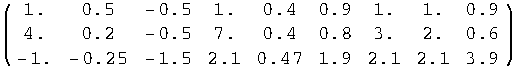
\includegraphics{refHmat.pdf}}}\intertext{with $\psi_c=\psi_\epsilon=0, \,\,  \psi_z=I$.
the series representation requires that the linear model
have a unique stable solution.}
  B=
\vcenter{\hbox{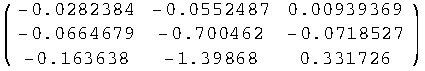
\includegraphics{refBmat.pdf}}}\\
\phi=
\vcenter{\hbox{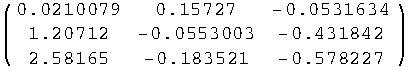
\includegraphics{refPhimat.pdf}}}\\
F=
\vcenter{\hbox{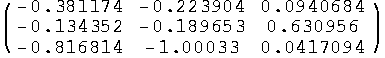
\includegraphics{refFmat.pdf}}}
\end{gather} 

\end{frame}
\subsection{Representing a Path}

\subsection{Representing a Family of Paths}

\subsection{Useful Properties of Series Solution}

\begin{itemize}
\item linear sum of functions
\item far away points matter less
\item Bounds on errors
\end{itemize}


\section{An RBC Model Example}
\subsection{Known Solution: Conditional Expectations Path}
\begin{itemize}
\item can easily compute series
\item algorithm can recover known solution
\end{itemize}


\subsection{UnKnown Solution: Conditional Expectations Path}
\begin{itemize}
\item can discover unknown solutions
\end{itemize}



\subsection{Occassionally Binding Constraints}
\begin{itemize}
\item can discover unknown solutions
\end{itemize}



\subsection{Regime Switching}
\begin{itemize}
\item can discover unknown solutions
\end{itemize}


\subsection{Regime Switching with Occassionally Binding Constraints}
\begin{itemize}
\item can discover unknown solutions
\end{itemize}

\section{Future Directions}

\begin{frame}
  \frametitle{Future Directions}
  \begin{itemize}
  \item Heterogeneous Agents Problems
  \item Convergence Properties
    \begin{itemize}
    \item no solution
    \item multiple solutions
    \end{itemize}
\item algorithmic details
  \begin{itemize}
 \item Smolyak nodes
 \item Projection Methods
 \item Perturbation Methods for initial guess
  \end{itemize}
\item Insights for ``pruning''
  \end{itemize}
\end{frame}

\begin{frame}
  \frametitle{Bibliography}
  \bibliographystyle{plainnat}
\bibliography{anderson,files}

\end{frame}



\end{document}
